%!TEX root=../document.tex
\section{Versuche}
\label{sec:Versuche}
Der erste Schritt für mich war es, es zu schaffen eine Demo laufen zu lassen. Am leichtesten lässt sich eine Demo ausführen, indem man eine Docker Instanz erstellt auf welcher ein vorkonfiguriertes image vorhanden ist. 

\subsection{cas-webapp-docker}
\cite{Apereio}

Dies ist das offizielle GitHub repository von Apereo, um eine demo webapp in einer Docker Instanz laufen zu lassen.

\subsubsection{Konfiguration}
Zuerst muss natürlich das repository geklont werden:
\begin{lstlisting}[language=bash]
	git clone https://github.com/apereo/cas-webapp-docker
\end{lstlisting}

Der nächste Schritt ist es, das docker Konfigurationsfile, \verb|Dockerfile|, anzupassen.

Hierbei muss vor allem darauf geachtet werden, dass das richtige \textbf{CAS Overlay Project} verwendet wird. D.h. es muss auf das CAS Overlay repository\cite{Apereo} gegangen werden, und die letzte Version in das \verb|Dockerfile| eintragen.

\subsubsection{Build}
Nun muss das projekt gebuilded und ausgeführt werden. Dies funktioniert über die beiden Shell-Scripts \verb|build.sh| und \verb|run.sh|. Beide werden mit einem Parameter gestartet, \textbf{\$CasVersion}, welcher bei beiden unbedingt gleich sein muss! Die tatsächliche Ausführung sieht dann beispielsweise folgendermaßen aus:

\begin{lstlisting}[language=bash]
./build.sh 1.0
./run.sh 1.0
\end{lstlisting}

\subsubsection{Probleme}
Das erste Problem war es, das README vom Repository zu verstehen. Es sind sehr viele wage Begriffe vorhanden und ich weiß noch immer nicht was genau es mit \$CasVersion auf sich hat.


Das Hauptproblem war nun, wenn die Instanz gestartet wird, wird folgender Fehler ausgegeben:

\begin{minipage}{\linewidth}
	\centering
	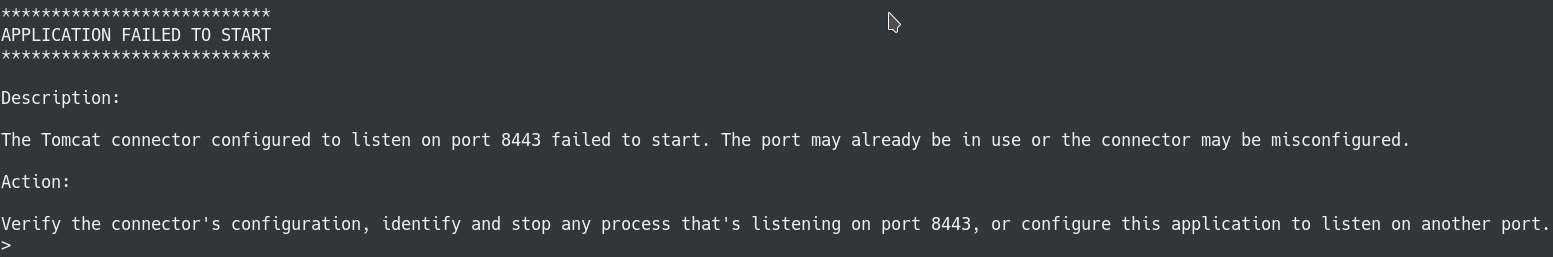
\includegraphics[width=1\linewidth]{images/failed_1}
	\figcaption{Fehler bei der Ausführung des Projekt cas-webapp-docker}
\end{minipage}

\subsubsection{Lösungsversuche}
Der erste Versuch war, da die Fehlernachricht sagt der Port sei besetzt, den Port 8443 frei zu machen. Doch der Befehl \verb=ss -lntu | grep 8443= gab nichts aus, also ist der Port definitv frei.

Ein weiteres Problem könnte im Dockerfile sein, zuerst habe ich Versucht die Java Versionen anzupassen da diese nicht mit meinem lokalen System übereingestimmt haben, aber nach der Erkenntnis das in einer abgekapselten Docker-Instanz gearbeitet wird, habe ich realisiert das es nicht an diesen Einstellungen liegen kann.

Tatsächlich wurde aber 10 Stunden vor der Labor-Einheit ein Issue\cite{Deric-dominic} in dem Repository gepostet, welches die exakt gleiche Fehlermeldung hat!

\subsection{cas}
\cite{Apereoa}

Das offizielle Cas Repository von Apereo, um einen CAS Server lokal aufsetzen zu können
\subsubsection{Konfiguration}
\cite{Apereob}

Das Problem hier bei ist, dass diese Konfiguration von einer lokalen Installation auf der Maschine ausgeht. Da das Ziel ist, eine dockerized-Installation aufzusetzen, war diese Dokumentation nicht sehr hilfreich.

\subsubsection{Probleme}
Es gibt zwar ein docker Ordner in dem Repository, aber in diesem ist kein \verb|README.md| vorhanden, um zu verstehen wie die docker-Instanz gestartet werden muss. 

\subsection{cas-overlay-demo}
\cite{Casinthecloud}

Dies ist ein Projekt, mit dem Ziel eine Demo-webapp mit dem \textbf{Maven Overlay} laufen zu lassen.

\subsubsection{Konfiguration}
Da dies ein komplett vorgefertiges, und leicht deploybares maven Projekt ist, sollte keine Konfiguration benötigt werden.

\clearpage
\subsubsection{Build}
Der einzige command der ausgeführt werden muss, um das Projekt zu starten ist:

\begin{lstlisting}[language=bash]
mvn clean install
\end{lstlisting}

\subsubsection{Probleme}
Das Projekt wurde erfolgreich installiert, nur ist das Problem für mich nun - was jetzt?
In der Dokumentation steht folgender Ausschnitt:

''
[..] and launch the CAS webapps via your favorite web application server with -Dcas.standalone.config=cas-overlay-server-demo/config.
''

\subsection{cas-overlay-docker}
\cite{Crpeck}

Dieses Projekt ist eine weitere Implementation des Overlay Mechanismus in CAS.

\subsubsection{Konfiguration}
Die docker-Instanz ist bereits vorkonfiguriert und sollte nur auszuführen sein mit:

\begin{lstlisting}[language=bash]
	docker-compose up --force-recreate
\end{lstlisting}

\subsubsection{Probleme}
Gleich bei der Ausführung des Befehls, wird eine Fehlermeldung ausgegeben:

\begin{minipage}{\linewidth}
	\centering
	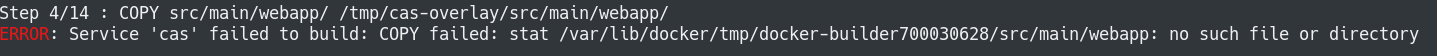
\includegraphics[width=1\linewidth]{images/failed_2}
	\figcaption{Fehler bei der Ausführung des Projekt cas-overlay-docker}
\end{minipage}

\subsection{docker-cas}
\cite{Terranex}

Eine weitere docker Implementation von CAS, mit der zusätzlichen Funktion eine Anmeldungsdelegation installiert bzw. konfiguriert zu haben, mit welcher sich über Facebook, Twitter und OpenID Connect zur webapp verbinden könnte.

\subsubsection{Build \& Konfiguration}
Nachdem \verb|build.sh| ausgeführt wurde, gibt es Files welche zum konfigurieren sind: \verb|cas.properties|, \verb|pac4jContext.xml| und \verb|server.xml|.

In \verb|server.xml| kann der Hostname und der Port des Server geändert werden.

In \verb|pac4jContext.xml| kann die Authentifikation via den 3rd-party Diensten konfiguriert werden. Da ich nicht sicher war, wie diese Anmeldungen über das Schul-WLAN funktionieren würden, habe ich sie deaktiviert indem ich die Einträge bei \verb|cas.pac4j| auskommentiert habe.

\subsubsection{Run}
Nun muss einfach nur \verb|run.sh| ausgeführt werden:

\begin{lstlisting}[language=bash]
./run.sh
\end{lstlisting}

Es müsste nun einfach auf die vorkonfigurierte Adresse (default \textbf{localhost:8080}) gegangen, und dann sollte der login via dem CAS Service funktionieren

\subsubsection{Probleme}
Das problem hierbei war komplex und versteckt. Der build hat gut funktioniert, doch nachdem versucht wird in die docker-Instanz zu wechseln, wird ein Fehler ausgegeben, dass das Image (\textbf{tb4mmaggots/tomcat}) weder \textbf{local} noch \textbf{remote} vorhanden ist. Es wird aufgefordert sich anzumelden, um das Image vom remote-Server zu beziehen, aber tatsächlich bin ich schon angemeldet. 

Bei der Suche nach diesem Image, hat sich herausgestellt, dass das Projekt vor 2 Jahren erstellt wurde, und anscheinend in diesem Zeitbereich das verwendete Image von docker-hub gelöscht wurde, da es vom Benutzer \textbf{tb4mmaggots} nur folgende Images gibt:

\begin{minipage}{\linewidth}
	\centering
	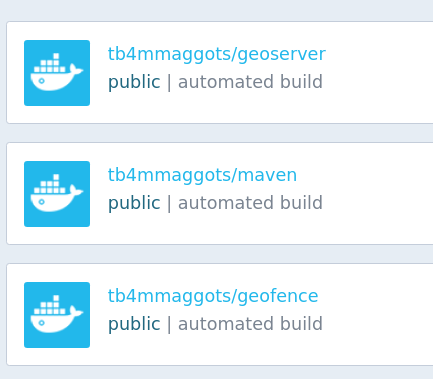
\includegraphics[width=0.5\linewidth]{images/failed_3}
	\figcaption{Verfügbare images von tb4mmaggots}
\end{minipage}

\subsubsection{Lösungsversuche}
Der erste versuch war es, statt dem vorkonfigurierten image von tb4mmaggots, einfach ein normales tomcat image zu verwenden. Es hat funktioniert, die docker-instanz zu starten und auch in diese zu wechseln, aber auf dem nun verwendeten image ist nun kein CAS-Server installiert oder konfiguriert. 

Weiter wurde versucht der \textbf{tb4mmaggots/geoserver} und \textbf{tb4mmaggots/maven} verwendet, aber beide images haben sich für diesen Zweck als nutzlos herausgestellt.

\section{Ergebnisse}
\label{sec:Ergebnisse}
\subsection{dockerized-cas}
\cite{J-fuentes}

Diese Projekt bietet, so wie viele andere bereits erwähnte Projekte, ein bereits vorkonfiguriertes image an welches mit docker ausgeführt werden kann.

\subsubsection{Run}
Es ist nichts zu konfigurieren, es muss lediglich folgendes ausgeführt werden:

\begin{lstlisting}[language=bash]
docker-compose up
\end{lstlisting}

Es sollte nun folgendes in der Konsole zu sehen sein:

\begin{minipage}{\linewidth}
	\centering
	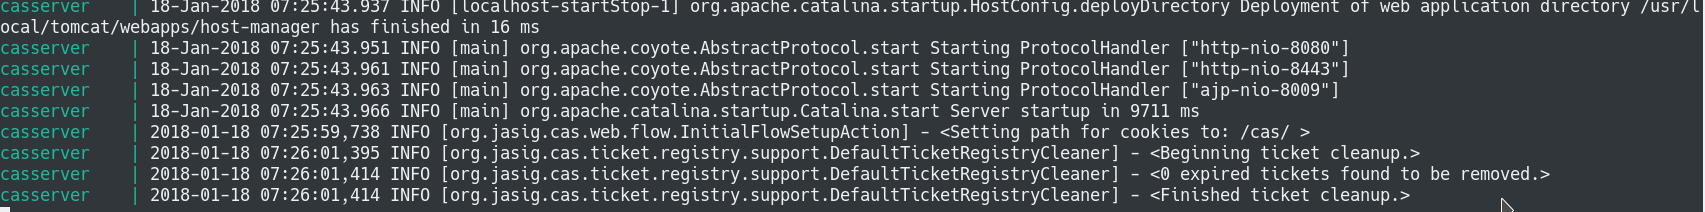
\includegraphics[width=1\linewidth]{images/funzt_1}
	\figcaption{Tomcat Server wurde gestartet}
\end{minipage}

\clearpage

\subsubsection{Testing}
Es wird nun auf \textbf{localhost:8080/cas} und man kann folgendes sehen:

\begin{minipage}{\linewidth}
	\centering
	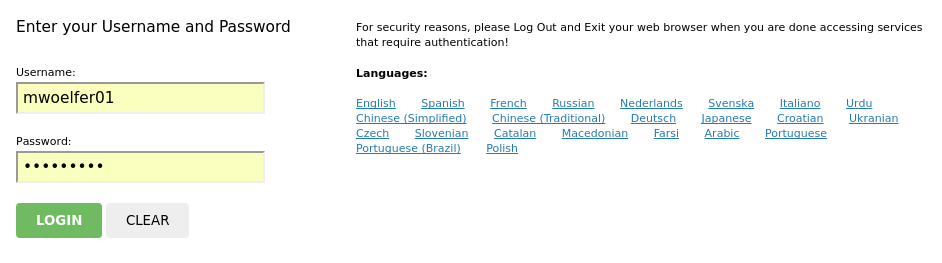
\includegraphics[width=1\linewidth]{images/funzt_2}
	\figcaption{Login ist möglich auf Tomcat Server via CAS}
\end{minipage}

In der Dokumentation steht, das sich mit folgendem User anzumelden ist:

\begin{itemize}
	\item User: casuser
	\item Password: Mellon
\end{itemize}

Bei der richtigen Angabe der Werte wird folgendes Ausgegeben:

\begin{minipage}{\linewidth}
	\centering
	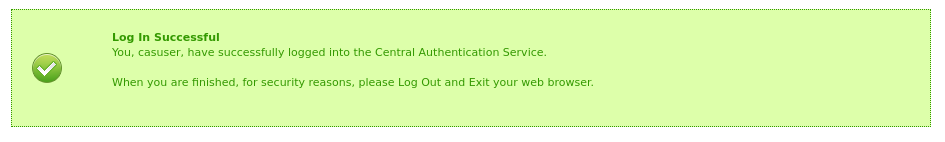
\includegraphics[width=1\linewidth]{images/funzt_3}
	\figcaption{Login via CAS ist erfolgreich}
\end{minipage}

Bei falschen Anmeldedaten gibt es folgende Ausgabe:

\begin{minipage}{\linewidth}
	\centering
	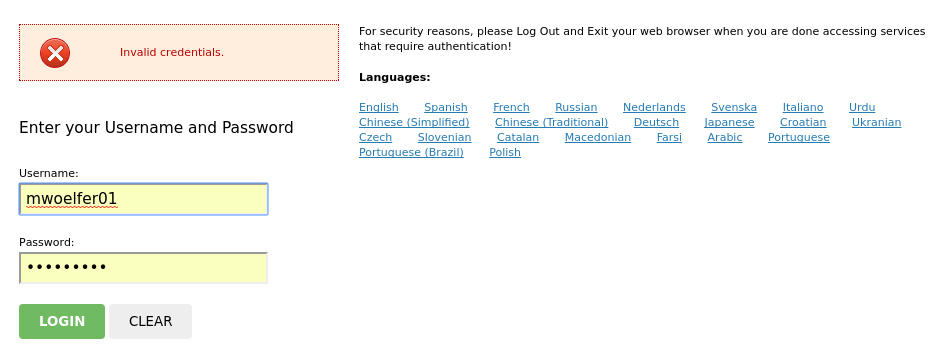
\includegraphics[width=1\linewidth]{images/funzt_4}
	\figcaption{Login via CAS ist fehlgeschlagen}
\end{minipage}